

\chapter{Creación del Proyecto}


En Chile, los Tribunales Ambientales son órganos jurisdiccionales especiales, sujetos a la 
superintendencia directiva, correccional y económica de la Corte Suprema, cuya función 
es resolver las controversias medioambientales de su competencia y ocuparse de los 
demás asuntos que la ley somete a su conocimiento \cite{Ley20600}. Estos tribunales generan una gran cantidad 
de jurisprudencia debido a los procesos como demandas, reclamaciones, etc. Que ellos atienden continuamente 
y que a su vez pueden ser encontrada en su portal de consulta llamado buscador ambiental \cite{BuscadorAmbiental}. 

Esta tesis contempla un proyecto consistente en la generación de un chatbot, donde se pueda preguntar sobre 
la jurisprudencia de los tribunales anteriormente descritos, por parte de cualquier persona sin necesidad de 
contar con una mucha expertiz en el ambito legal. Sin embargo, por razones de capacidad de computo y limitaciones 
de la tecnología el chatbot se 
vera acotado en sus capacidades a solamente procesar las reclamaciones recibidas por el tribunal y no otro tipo d
e litigios que pueda antender dicho tribunal. Para este chatbot, se considero una estructura como 
la representada en la \autoref{fig:estructura}.

El proyecto esta contruido por diferentes etapas que consisten en: un proceso de extracción de datos 
desde el buscador ambiental, otro de transformación de estos datos para su utilización, la generación 
de vectores de los datos transformados para que puedan interactuar con la aplicación, un carga de estos vectores 
en una base de datos, para que después el chatbot que se creara, pueda interactuar con ellos y mandandar 
esa información a el gran modelo de lenguaje (LLM), siendo en este caso el modelo ``gpt-4'' perteneciente a OpenAI,
 siendo la estrutura basica del proyecto la de \autoref{fig:estructura}.
% Inclusión de Figuras
\begin{figure}[ht!]
    \centering
    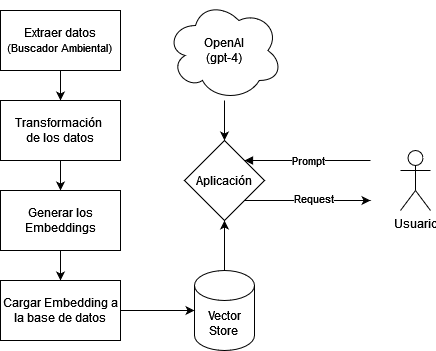
\includegraphics[width=.47\textwidth]{figures/huemul1.png}
    \caption[Estructura basica de la aplicación]{Estructura basica de la aplicación\\
    {\scriptsize (Fuente: Elaboración propia)}}
    \label{fig:estructura}
\end{figure}
    

A partir de esta estructura basica anteriormente mencionada en la \autoref{fig:estructura}, se explicará parte 
por parte el proceso con mucha mas profundidad cosa de entender tanto el funcionamiento como el proceso de creación, 
por lo que para empezar se iniciara con el proceso de ETL.



\section{ETL}


Para realizar la realizacipon del proyecto, fue necesario realizar un proceso de ETL. El término ETL se refiere a las técnicas de "Extracción, 
Transformación y Carga" (Extract, Transform, Load), que constituyen un proceso clave para los datos necesarios para el proyecto. 
Este proceso implica la extracción de datos de fuentes heterogéneas, su transformación para ajustarse a las necesidades del 
negocio y su posterior carga en un destino que, por lo general, es un almacén de datos diseñado para el análisis y la generación 
de informes o aplicaciones \cite{ETL1}. Siendo en este proyecto el proceso como el que se muestra en la \autoref{fig:etl1}.

% Inclusión de Figuras
\begin{figure}[ht!]
    \centering
    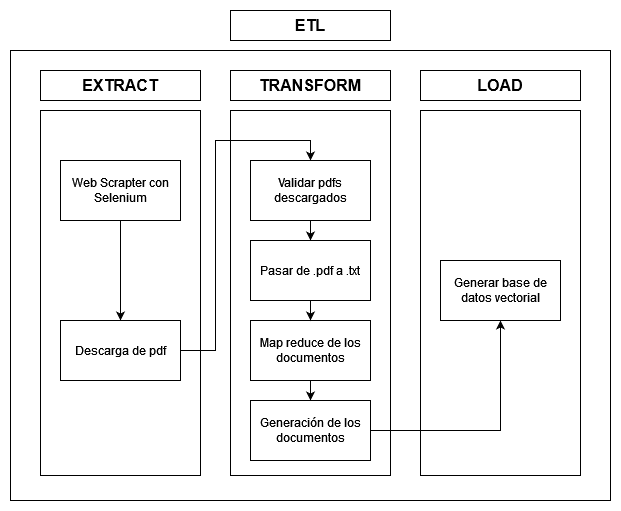
\includegraphics[width=.7\textwidth]{figures/huemulETL.png}
    \caption[Estructura del proceso de ETL para el Buscador Ambiental]{Estructura del proceso de ETL para el Buscador Ambiental\\
    {\scriptsize (Fuente: Elaboración propia)}}
    \label{fig:etl1}
\end{figure}
    

Para la fase de extracción de los datos, esta implica la recolección de datos de múltiples fuentes, que pueden variar desde bases de datos 
estructuradas hasta información no estructurada en la web u otra fuente. La transformación se refiere al proceso de limpieza, conversión, 
y consolidación de estos datos en un formato adecuado para el análisis o entendimiento de la aplicación que se usara. Finalmente, la carga es el proceso de transferir 
los datos transformados al sistema de destino, donde se pueden almacenar y utilizar para la toma de decisiones estratégicas 
\cite{ETL1}.

\subsection{Extract}

Iniciando la extracción de los datos, la información requerida para el desarrollo del Chatbot se obtuvo del ``Buscador ambienta'' del Tribunal de Protección Ambiental 
de Chile a través de su sitio web \cite{BuscadorAmbiental}. Este portal aloja todos los documentos públicos disponibles para su consulta en cualquiera 
de los tres tribunales ambientales. Para acceder a la base de datos necesaria y extraer el contenido necesario, se llevó a cabo la creación de 
un bot, definiendo un bot como un programa de software automatico, repetitivo y con tareas predefinidas \cite{Kaspersky_2023}, capaz de recopilar
de manera automatica cada una de las entradas de este buscador, de manera análoga a cualquier usuario convencional
que consultaria una jurisprudencia en el buscador.

\begin{figure}[ht!]
    \centering
    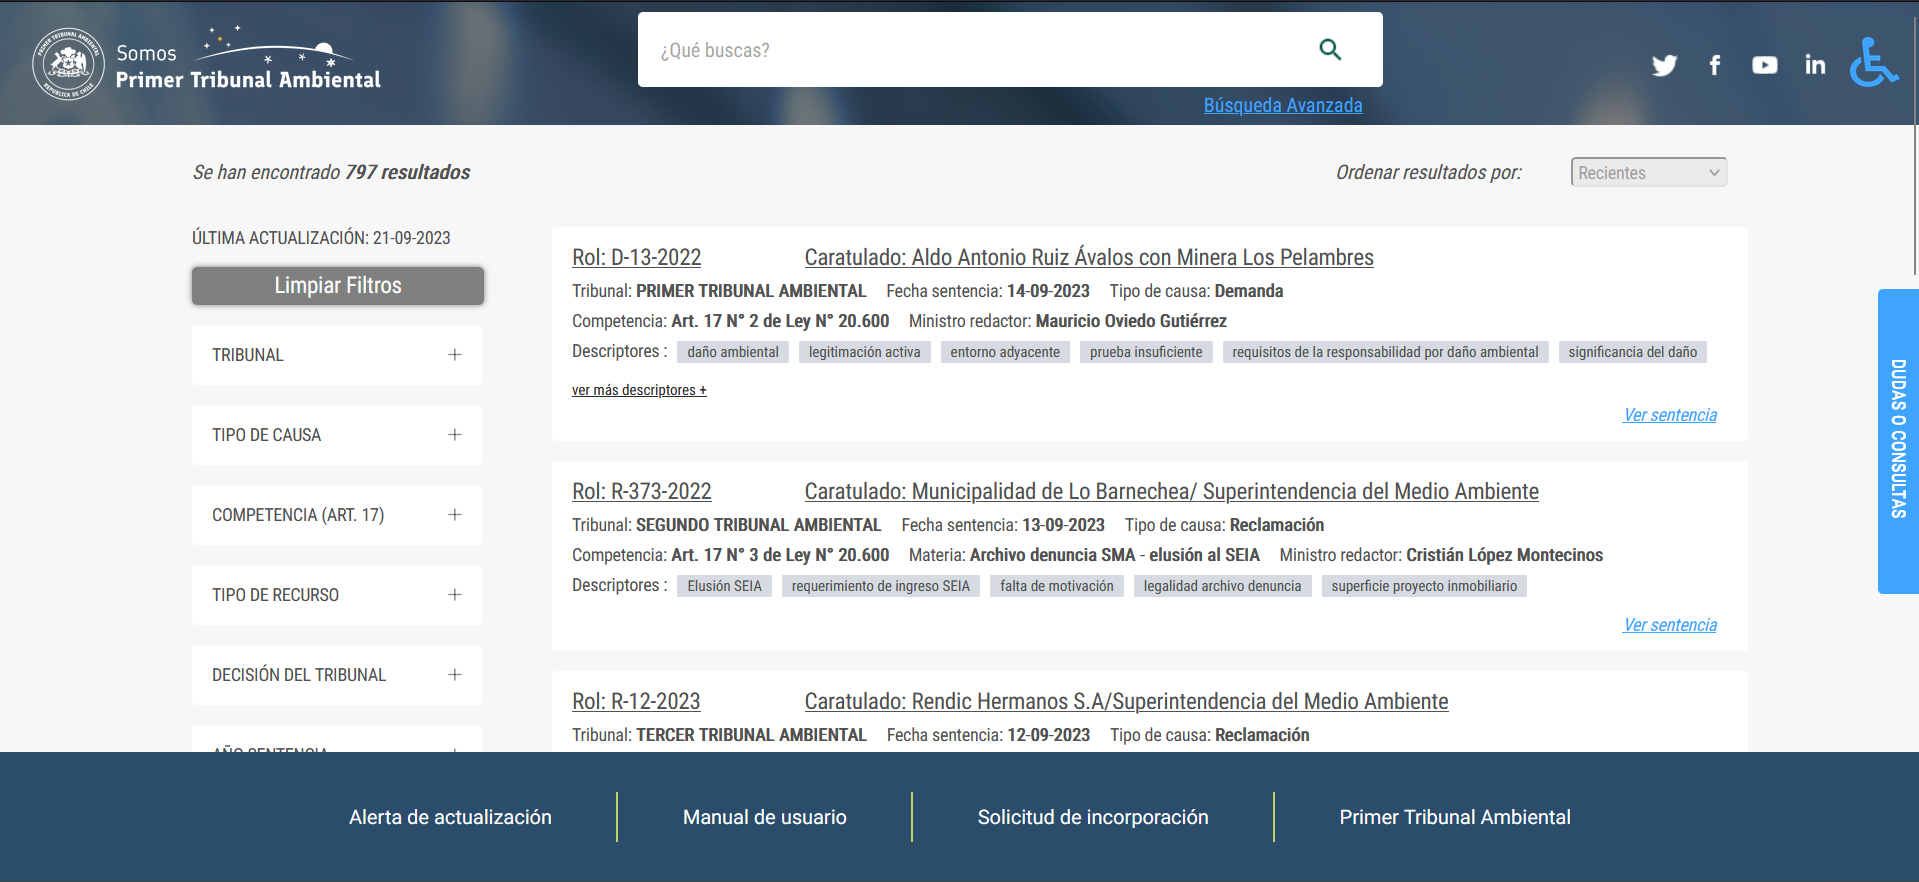
\includegraphics[width=.75\textwidth]{figures/huemul2.png}
    \caption[Screenshot del Buscador de la pagina del Primer Tribunal Ambiental]{Buscador de la pagina del Primer Tribunal Ambiental\\
    {\scriptsize (Fuente: Pagina del Primer Tribunal Ambiental)}}
    \label{fig:extract1}
\end{figure}
    
Para esta tarea, se empleó Selenium \cite{seleniumSelenium}, una herramienta originalmente diseñada para generar pruebas unitarias en software, pero que, debido a la naturaleza 
reactiva y dinámica de los sitios web, así como la activa detección de bots por parte de algunas páginas, resulta ser la elección 
más apropiada para la extracción de datos del buscador. Este bot, después de explorar cada una las páginas del buscador ambiental, como se ilustra en la \autoref{fig:extract1},
logro recolectar cada uno de los enlaces individuales que conducen a las páginas específicas de cada caso, tal como se 
muestra en la \autoref{fig:extract2}, para de ellas luego extraer más información.

\begin{figure}[ht!]
    \centering
    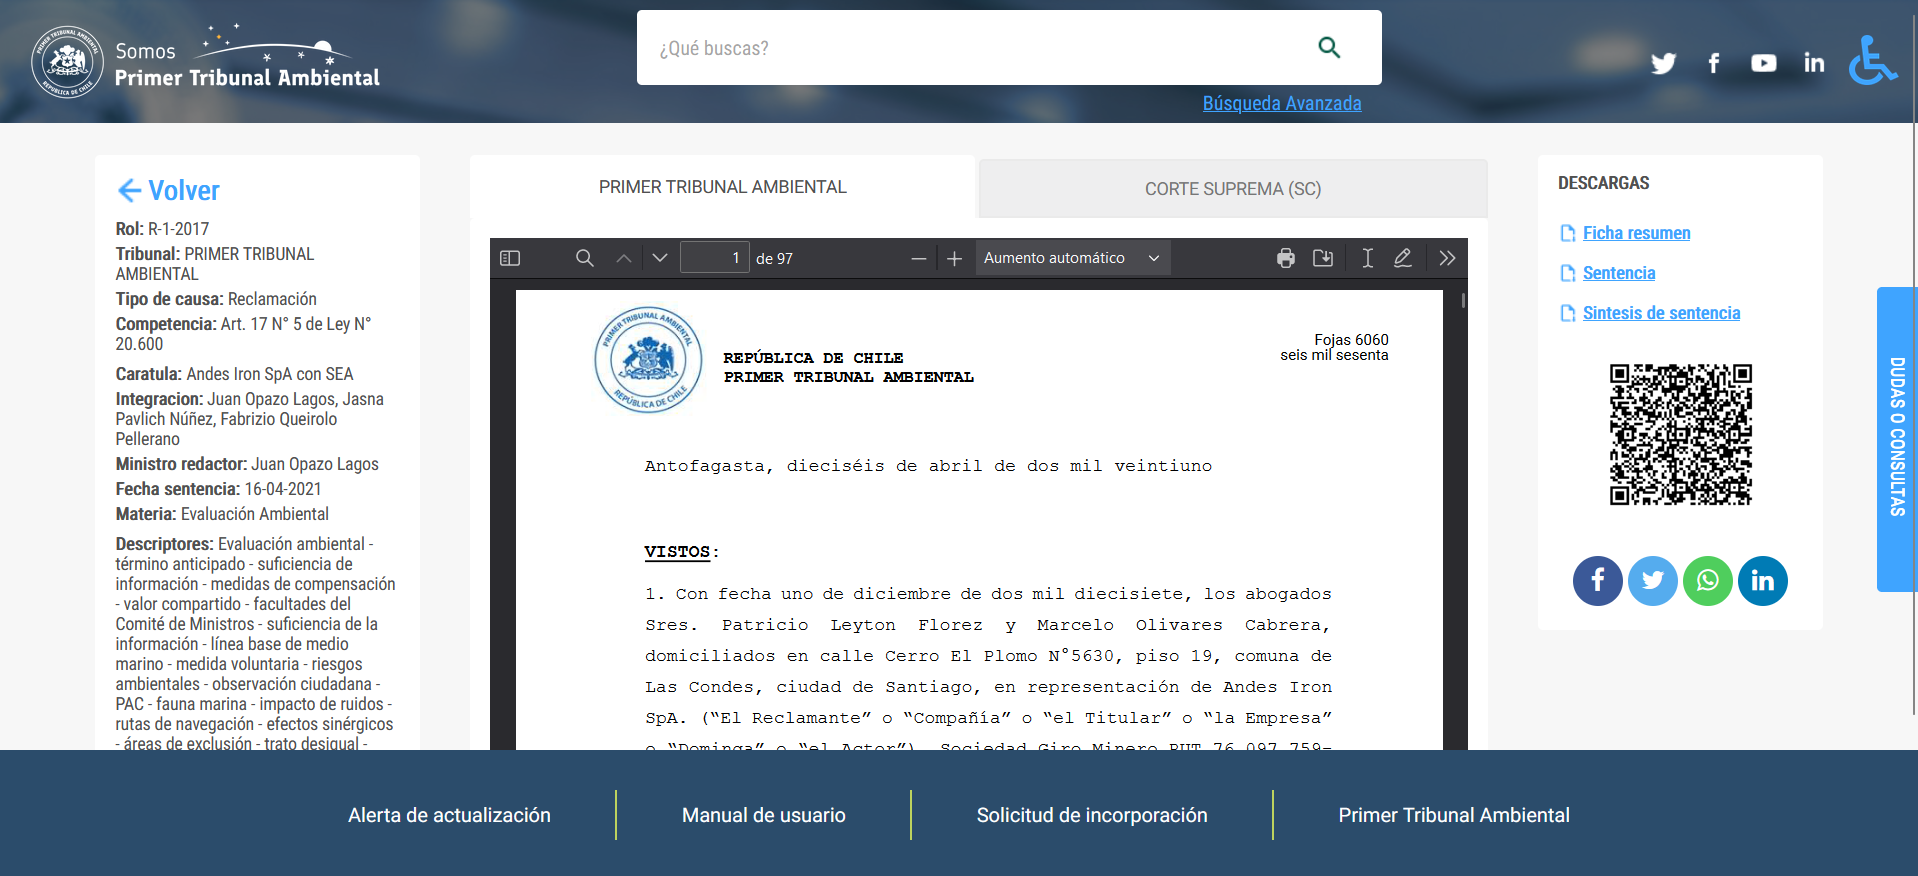
\includegraphics[width=.75\textwidth]{figures/huemul3.png}
    \caption[Screenshot de una sola reclamación en la pagina web del buscador ambiental]{Screenshot de una sola reclamación en la pagina web del buscador ambiental\\
    {\scriptsize (Fuente: Pagina del Primer Tribunal Ambiental)}}
    \label{fig:extract2}
\end{figure}

\newpage

Posteriormente, se contemplo la posibilidad de obtener tanto los enlaces a cada documento en formato PDF como la información 
detallada de cada uno de estos documentos, pudiendo llamar a esta información metadata, mediante la creación de un nuevo bot. 
Sin embargo, durante el proceso de desarrollo de este bot, se logró utilizar el mismo bot anteriormente usado, pero modificandolo,
por lo que al hacerlo permitía obtener todos los datos mencionados anteriormente. Esto suprimió 
la necesidad de crear otro tipo de bot utilizando Selenium, ya que esta modificacion logro obtener dichos resultados.

Para completar la fase de extracción de datos (Extract), una vez que se había obtenido toda la información mediante este bot con Selenium, 
el último paso consistió en generar un script, definiendo script como una serie de intrucciones de son interpretas por un programa \cite{techtargetWhatScript}, que generara nuevas solicitudes con el objetivo de descargar todos los archivos PDF de cada una 
de las entradas del buscador. 
Como una limitación a la extracción de datos se decidió solo descargar las reclamaciones e ignorar el resto de los documentos que recibe el tribunal ambiental, cosa de acotar el proyecto en si y a limitaciones de parte del poder computacional que se dispuso a la hora de escribir esta tesis.
Estos archivos luego de ser descargados, estan listos para la próxima etapa del proyecto, que implica la transformación 
de los datos con el fin de procesar esta información, que luego sera necesaria para construir la base de datos a partir de los documentos descargados.
Dejando todo el proceso de ``Extract'' como se muestra en la \autoref{fig:extract_diagram}. 

\begin{figure}[ht!]
    \centering
    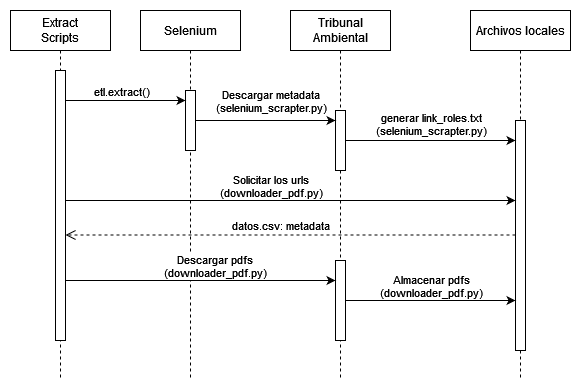
\includegraphics[width=0.9\textwidth]{figures/extract_diagram.png}
    \caption[Diagrama de secuencia para el proceso de extracción (Extract) de datos del proyecto]{Diagrama de secuencia para el proceso de extracción (Extract) de datos del proyecto\\
    {\scriptsize (Fuente: Elavoración propia)}}
    \label{fig:extract_diagram}
\end{figure}


\newpage

\subsection{Transform}

% CHAGO: Ojo lo de semejanza semantica
\par Continuando con el proceso de ETL, los PDFs que previamente habian sido descargados en el proceso de Extract,
ahora requieren ser sometidos a modificaciones en la estructura y formato de sus datos, con el objetivo de convertir la información que inicialmente se presenta en un 
estado ``sucio'' a uno  ``limpios'' cosa que puedan ser usados adecuadamente dentro posteriores tareas del proyecto. A esta serie de actividades de modificaciones a los datos lo denominamos
``Transformación'', o ``Transform,'' en inglés.

\par Entre los datos descargados, nos encontramos con un extenso número de PDFs que presentan una serie de dificultades significativas para su 
manipulación dentro del programa. Esto se debe a que el Tribunal Ambiental no sigue un formato estándar en la estructura de las reclamaciones 
presentadas. En consecuencia, cada uno de los textos posee un formato propio, lo que complica en gran medida la extracción 
eficiente de las diversas secciones contenidas en dichos textos. Sin embargo, gracias al funcionamiento del proceso de semejanza 
semántica que se empleara por el chatbot, esta diversidad de formatos no representa un problema insuperable para el proyecto.

\par No obstante, surgen dificultades adicionales cuando se trata de las reclamaciones que son presentadas a los tribunales ambientales 
en formato digital o, en su defecto, en forma de fotocopias. Esto implica que no todos los documentos están habilitados para su 
procesamiento y con ello la extracción de su información. En consecuencia, el primer paso en el proceso de transformación involucra la discriminación de qué PDFs son 
susceptibles de ser procesados y cuáles no. Para llevar a cabo esta tarea, se ha desarrollado un script capaz de detectar 
texto dentro de un archivo PDF. Si el texto es legible, se almacena; de lo contrario, se elimina de los archivos descargados.

\par Una vez separados los PDFs legibles y adecuados para el trabajo posterior, se procedio con la transformación de estos documentos 
al formato TXT (texto plano). Esta etapa se realizo, considerando la conveniencia de trabajar con archivos en formato de 
texto en comparación con los archivos en formato PDF puro, dado que el próximo método de transformación, que implica el uso de
map-reduce utilizados por Langchain, requiere que los datos estén en formato que sea interpretable por el framework.

 \begin{figure}[ht!]
    \centering
    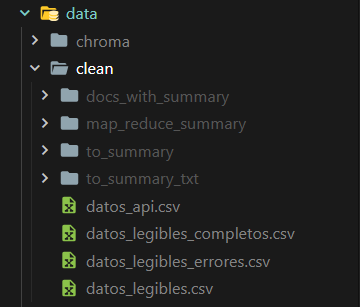
\includegraphics[width=.5\textwidth]{figures/huemulFOLDERS.png}
    \caption[Estructura de carpetas y datos del proyecto]{Estructura de carpetas y datos del proyecto]\\
    {\scriptsize (Fuente: Elavoración propia)}}
    \label{fig:chatbot1}
\end{figure}

\newpage

\par El funcionamiento interno de tanto el proceso de ETL como el futuro Chatbot, se basa en el framework Langchain para la interacción con el Modelo de Lenguaje Grande (LLM). 
LangChain es un framework poderoso que simplifica el desarrollo de aplicaciones utilizando modelos de lenguaje grandes (LLM). Proporciona 
una interfaz única y personalizable capaz de gestionar diferentes LLM, incluida la gestión rápida, el procesamiento, el aumento de datos, 
la orquestación de agentes, el almacenamiento y la evaluación. Este marco versátil permite a los desarrolladores integrar perfectamente 
los LLM con sus flujos de trabajo del mundo real y datos con el mínimo esfuerzo \cite{langchain1}.



\par El proceso de Map-Reduce llebado a cabo por Langchain, es un modelo de programación diseñado para procesar grandes cantidades de datos de manera eficiente, 
escalable y distribuida a través de clústeres de servidores. En el contexto de un archivo PDF muy extenso, por ejemplo, si se requiere resumir 
el contenido o analizar la frecuencia de ciertas palabras, Map-Reduce podría ser utilizado para dividir la tarea en partes más pequeñas y manejables. Siguiendo con el ejemplo del PDF extenso
en primera instancia, la función de map tomaría el texto del PDF y lo dividiría en elementos más pequeños, como párrafos o líneas, 
asignando a cada uno un resumen intermedio \cite{mapreduce}. Luego, la función reduce recogería todos los resumenes intermedios asociados con el documento extenso
y los combinaría para producir un resultado agregado, con un resumen de todo el documento. 

\begin{figure}[ht!]
    \centering
    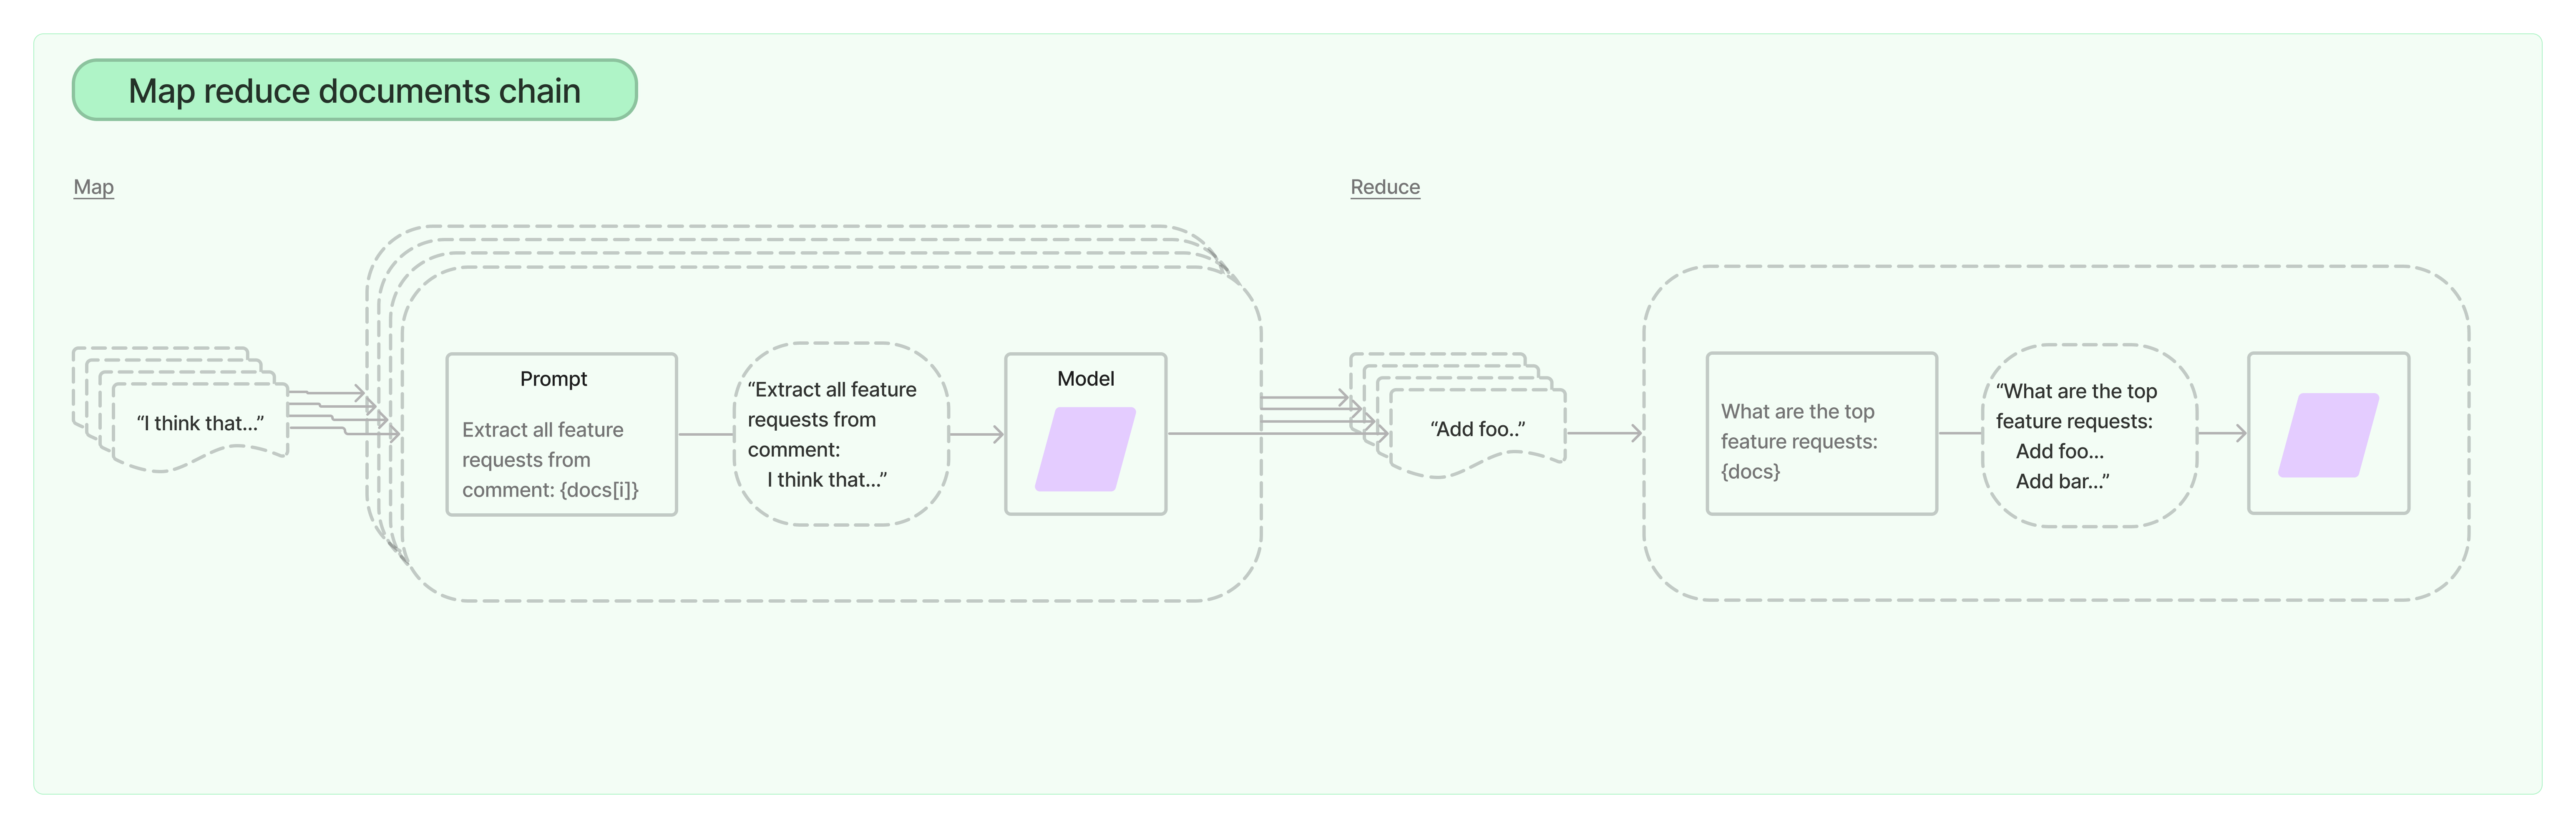
\includegraphics[width=1\textwidth]{figures/huemul_mapreduce.jpg}
    \caption[Diagrama de funcionamiento de la función mapreduce en un documento]{Diagrama de funcionamiento de la función mapreduce en un documento\\
    {\scriptsize (Fuente: Langchain \cite{framework1})}}
    \label{fig:chatbot1}
\end{figure}

\par Continuando el con el proceso de transform y entrando a un proceso de map-reduce, es importante destacar que un archivo .txt obtenido del proceso anterior, 
puede contener una extensión demasiado grande, lo que conlleva a que tenga número de tokens muy elevado como para ser reducido de manera inmediata. 
En situaciones de este tipo, es necesario recurrir a un proceso de subdivisión que fragmenten los textos en segmentos con un número de tokens inferior al límite impuesto por 
la API OpenAI a los modelos de LLM de la empresa, siendo en este caso el modelo ``gpt-4'' que tiene un limite de 8,192 tokens por llamada a la API \cite{openaimodels}.
Cada archivo .txt puede ser dividido, resumido y exportado a un nuevo archivo .txt una vez que ha sido fragmentado previamente en segmentos.

\newpage

\par Los documentos procesados son combinados utilizando otro proceso por parte de Langchain, cosa obtener un resultado final con toda la datos de los documentos consolidados. 
Para concluir el proceso de transformación, los resúmenes generados después de haber pasado por el procedimiento de map-reduce 
se someten a una última tarea, antes de ser incorporados en la base de datos mediante el el proceso de ``load''. Este paso implica la fusión de los resúmenes con la 
información obtenida a través de la información extraida por Selenium previamente y que es especifica de cada texto llamada metadata, la cual es añadida a cada documento final en forma de texto. Este proceso 
resulta en la creación de un único documento para cada reclamación que engloba toda la información pertinete a ella, a los cuales nos referiremos como ``documentos finales''. 
Con esto, se concluye la fase de transformación y se procede al último procedimiento, conocido como ``carga'' (Load), que consiste 
en el almacenamiento estos documentos finales en la base de datos. Dejando todo el proceso de ``Transform'' como se muestra en la \autoref{fig:transform_diagram}. \\


\begin{figure}[ht!]
    \centering
    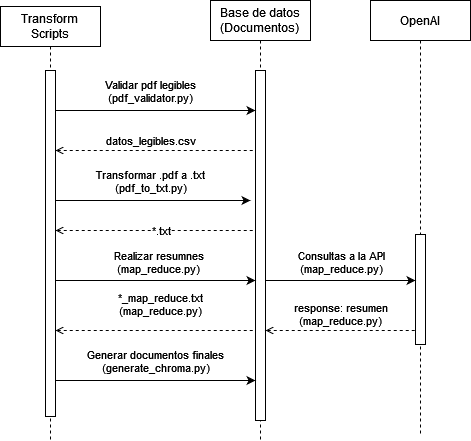
\includegraphics[width=0.8\textwidth]{figures/transfrom_diagram.png}
    \caption[Diagrama de secuencia para el proceso de transformación (Trasform) de datos]{Diagrama de secuencia para el proceso de transformación (Trasform) de datos\\
    {\scriptsize (Fuente: Elavoración propia)}}
    \label{fig:transform_diagram}
\end{figure}


\newpage

\subsection{Load}

\par Al culminar el proceso de Extracción, Transformación y Carga (ETL), el siguiente y ultimo paso a llevar a cabo la fase de carga, 
también conocida como ``load'' en inglés, en la cual se incorporan todos los documentos previamente descargados y transformados 
en una base de datos. Para este proyecto, en el cual se utiliza LangChain, resulta de vital importancia fragmentar los documentos 
en secciones más pequeñas cosa que el Chatbot tenga la facilidad de consultar dichos fragmentos en un futuro, por lo que se deben dividir en fragmentos
mas pequeñoss todos los documentos los que llamaremos chunk.

\par Esta necesidad de dividir estos documentos, surge debido a que los documentos deben ser sometidos a un proceso de Embeddings, proceso que
previamente se explico en el estado del arte de esta tesis, antes de ser 
introducidos en la base de datos. Esto se debe principalmente a que las funciones de Embeddings tienen un límite en la extensión 
de grupos de caracteres, conocidos como ``tokens'', que pueden ser procesados a la vez. En el contexto del modelo de Embeddings que funciona
para el modelo de LLM ```gpt-4''' que utlizamos en este proyecto, se usa la función
``text-embedding-ada-002'' que cuenta con un límite que se establece en 8191 tokens \cite{openai1}, lo que constituye la longitud máxima de los fragmentos, o chunks, que
formaremos en el proceso de ``load''.

\par Por lo tanto, cuando se trabaja con documentos extensos, es indispensable dividirlos en fragmentos más pequeños antes de proceder 
con su incorporación, debido a las limitaciones de entrada en la ventana de contexto de los LLM, pues en este proyecto estos fragmentos despues seran enviados como contexto y este contexto no puede exceder dicha ventana. Según la información proporcionada en el Blog de OpenAI, los embeddings son ``representaciones numéricas 
de conceptos convertidos en secuencias numéricas, lo que facilita que las computadoras comprendan las relaciones entre los 
conceptos'' \cite{openai1}. En términos sencillos, los embeddings son representaciones vectoriales de texto que permiten su comprensión por 
parte de los Modelo de Grandes de Lenguaje (LLM). Dado que los LLM son redes neuronales, el proceso de Embedding resulta 
esencial para traducir el texto en números, que es el formato comprensible para esta red neuronal y permitir que el Chatbot funcione 
correctamente.

\par Langchain internamente, para llevar a cabo el proceso de carga de datos a la base de datos, toma todos los documentos finales proveniente del proceso de Transform en formato .txt y los divide en chunks que no superen la extensión máxima que puede procesar la función de embbedding de OpenAI, para luego enviar uno por uno dichos chunk mediante llamadas a la API de OpenAI, cosa de obtener los vectores asociados a cada uno de los textos enviados. 
Los vectores resultantes de enviar los chunks de documetos a la funcion de embeddings, se almacenan posteriormente en una base de datos vectorial llamada ChromaDB. Esta base de 
datos vectorial, también llamada vecto-store en ingles, ha sido diseñada para ser compacta, escalable y eficiente, con el propósito de almacenar y recuperar vectores de manera 
efectiva. ChromaDB genera índices que permiten una recuperación rápida y eficiente de los embeddings en función de las 
consultas realizadas por los usuarios \cite{langchain1}. Con ello, esta base de datos guarda los vectores asociados a el chunk de un documento, 
el texto del chunk del documento y su metada asociada.

\newpage

\par Con este último procedimiento se concluye el proceso de ETL para los datos del tribunal ambiental, procediendo de esa manera 
a la programación e implementación del Chatbot que usara estos datos para entregar respuesta sobre estos datos con el uso de 
lenguaje natural y con ellos dejando el proceso de ``load'' como se muestra en la \autoref{fig:load_diagram}.\\


\begin{figure}[ht!]
    \centering
    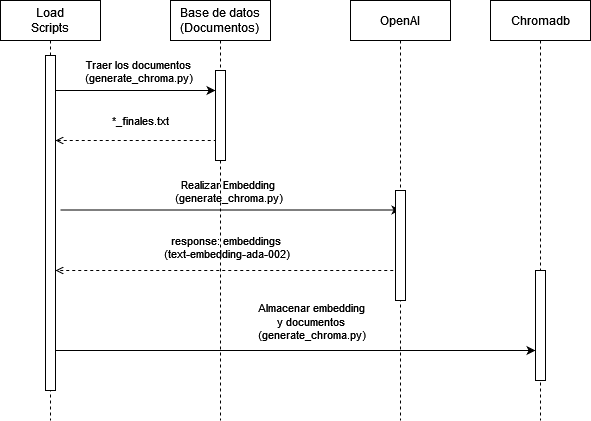
\includegraphics[width=0.8\textwidth]{figures/load_diagram.png}
    \caption[Diagrama de secuencia para el proceso de carga (Load) de datos]{Diagrama de secuencia para el proceso de carga (Load)  de datos\\
    {\scriptsize (Fuente: Elavoración propia)}}
    \label{fig:load_diagram}
\end{figure}

\newpage

\section{Chatbot}

   
La estructura del chatbot se desarrolló en su totalidad utilizando el lenguaje de programación Python. Esta elección se debió a la 
experiencia del equipo en Python, lo que facilitó tanto la creación del frontend como del backend de la aplicación.

Para la parte de la interacción del usuario (frontend), se empleó Python junto con el framework Flask para la presentación 
de contenido en pantalla, incluyendo tanto la estructura de HTML como las hojas de estilo CSS. Además, se aprovechó la potencia del 
framework Bootstrap para agilizar el proceso de maquetación.

En cuanto al backend, se implementó una API con el objetivo de facilitar la interacción entre el frontend y el backend. Para este 
propósito, se utilizó FastAPI, un framework que permite la creación rápida de APIs y que ofrece la ventaja de contar con Swagger 
para la prueba y generación automática de documentación.

\begin{figure}[ht!]
    \centering
    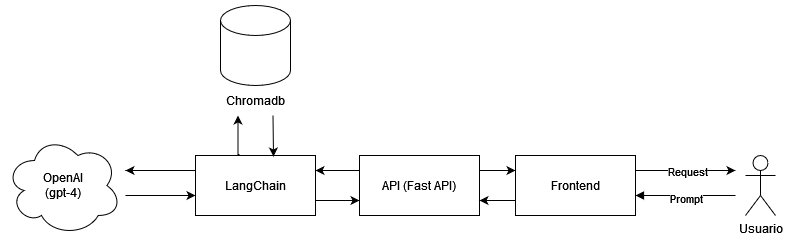
\includegraphics[width=.8\textwidth]{figures/finalhuemul.png}
    \caption[Diagrama de funcionamiento del Chatbot]{Diagrama de funcionamiento del Chatbot\\
    {\scriptsize (Fuente: Elavoración propia)}}
    \label{fig:chatbot1}
\end{figure}

% ELIMINAR
El funcionamiento interno de la aplicación se basa en el framework Langchain para la interacción con el Modelo de Lenguaje Grande (LLM). 
LangChain es un framework poderoso que simplifica el desarrollo de aplicaciones utilizando modelos de lenguaje grandes (LLM). Proporciona 
una interfaz única y personalizable capaz de gestionar diferentes LLM, incluida la gestión rápida, el procesamiento, el aumento de datos, 
la orquestación de agentes, el almacenamiento y la evaluación. Este marco versátil permite a los desarrolladores integrar perfectamente 
los LLM con sus flujos de trabajo del mundo real y datos con el mínimo esfuerzo \cite{langchain1}.
% ELIMINAR

Para la base de datos se utilizó ChromaDB. ChromaDB es una base de datos vectorial sin esquemas diseñada específicamente para 
su uso en aplicaciones de inteligencia artificial. Es liviano y muy potente, lo que permite el almacenamiento, la recuperación 
y la gestión eficiente de datos vectoriales (Embeddings), lo cual es esencial para las aplicaciones de chat de documentos 
basadas en LangChain y OpenAI \cite{langchain1}. Para que finalmente estas trabajaran en conjunto con los modelos de OpenAI, 
específicamente el modelo gpt-4 que actualmente es el más potente del mercado.

\begin{figure}[ht!]
    \centering
    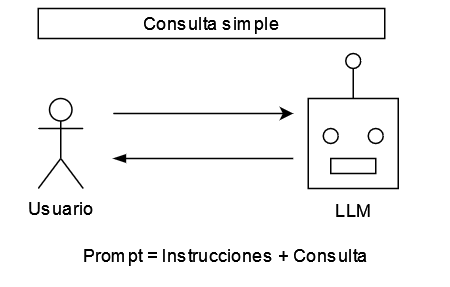
\includegraphics[width=.4\textwidth]{figures/huemul6.png}
    \caption[Diagrama en consulta simple]{Diagrama en consulta simple\\
    {\scriptsize (Fuente: Elavoración propia)}}
    \label{fig:chatbot1}
\end{figure}


La función principal del chatbot es generar respuestas utilizando la técnica "Retriever-Augmented Generation" (RAG), 
que implica proporcionar contexto adicional en el prompt enviado a OpenAI. Mientras que una generación simple suele 
constar de instrucciones y una consulta, en RAG se agrega contexto dentro del prompt con el propósito de reducir la 
probabilidad de alucinaciones y mejorar la calidad de las respuestas. 


En cambio, mediante ``Retriever-Augmented Generation'' 
consiste al igual que el proceso anterior en entregar las instrucciones y una consulta, pero junto ello se agrega un contexto 
de este, cosa de que el modelo largo de lenguaje tenga menor capacidad de alucinar y generar una mejor respuesta. Podemos decir
que ``Retriever-Augmented Generatio'' (RAG) se refiere a un modelo de generación de lenguaje que se mejora por la capacidad 
de recuperar información de una base de datos, como un índice de vectores que representan los documentos del buscador ambiental, 
además de la memoria que ya posee. Este enfoque se utiliza para mejorar la generación de respuestas en tareas de procesamiento 
de lenguaje natural (NLP) que requieren conocimiento intensivo \cite{raq}.

\begin{figure}[ht!]
    \centering
    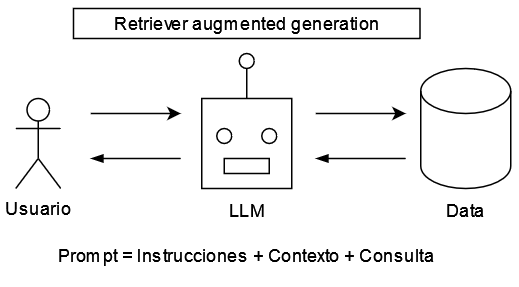
\includegraphics[width=.4\textwidth]{figures/huemul5.png}
    \caption[Diagrama en consulta mediante Retriver augmented generation]{Diagrama en consulta mediante Retriver augmented generation\\
    {\scriptsize (Fuente: Elavoración propia)}}
    \label{fig:chatbot1}
\end{figure}

Finalmente, este chatbot envía el prompt con las instrucciones y el contexto obtenido mediante el RAG realizado con 
Langchain a el LLM, siendo en este caso gpt-4 de OpenAI, luego de pasar por una función de Embedding, cosa de que 
pueda ser leído por el modelo. Por lo que se realiza un request con la información a la API de OpenAI, para que se 
obtenga el output con la respuesta.


Esta tesis se centra tanto en el riesgo\autoref{appx:contexto}. como en el desarrollo de un Chatbot, este chatbot funciona 
en base a la una arquitectura de RAG (Retriever-Augmented Generation) por lo que esta consiste en 
la recuperación de contexto el cual es enviado junto con el prompt al LLM. El proceso comienza con 
la obtención de un prompt específico del usuario, tal como ``Dame un resumen del documento Dominga'' 
dentro de la barra de búsqueda del frontend. Este prompt actúa como entrada inicial para el sistema 
de recuperación de información.

%\begin{figure}[ht!]
%    \centering
%    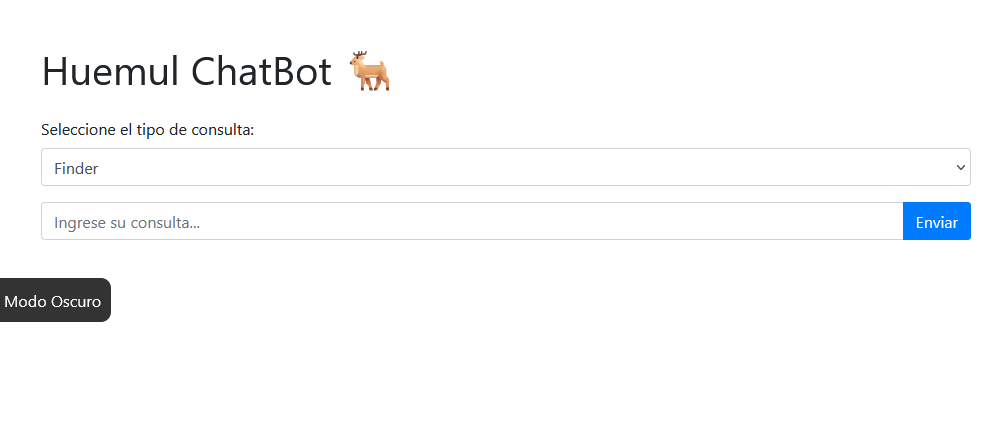
\includegraphics[width=.8\textwidth]{figures/website.png}
%    \caption[]{\\
%    {\scriptsize (Fuente: Elavoración propia)}}
%    \label{fig:chatbot1}
%\end{figure}

El prompt se procesa mediante una función de Embedding, empleando para ello OpenAI, siendo esta  
la función 'text-embedding-ada-002'. Esta función puede manejar hasta un máximo de 8191 tokens y 
produce un vector de 1536 dimensiones en forma de lista \cite{openai1}. Para determinar la similitud entre el 
vector del prompt y los vectores correspondientes a los documentos almacenados, se utiliza la función 
de similitud coseno presente en la \autoref{eq:similitudcoseno}.Esta mide el coseno del ángulo entre dos vectores,
Siendo estos $A$ y $B$ respectivamente, y este proporciona un valor que refleja su proximidad semántica entre el vector
del prompt y los vectores de todos los documentos almacenados en la base de datos ChromaDB.

\begin{equation}
    \text{similitud\_coseno}(\mathbf{A}, \mathbf{B}) = \frac{\mathbf{A} \cdot \mathbf{B}}{\|\mathbf{A}\| \|\mathbf{B}\|}
    \label{eq:similitudcoseno}
\end{equation}


El proceso de embedding como se menciono antes lo que realiza en otras palabras es la conversión de un texto a un vector, esto debido a que los modelos de LLM al ser basados 
en redes neuronales necesitan un presentación grafica de estos texto a un formato el cual pueda ser legible por el modelo, por lo que se convierten en números como muestra la 
\autoref{fig:caso1} a continuación.

\begin{figure}[ht!]
    \centering
    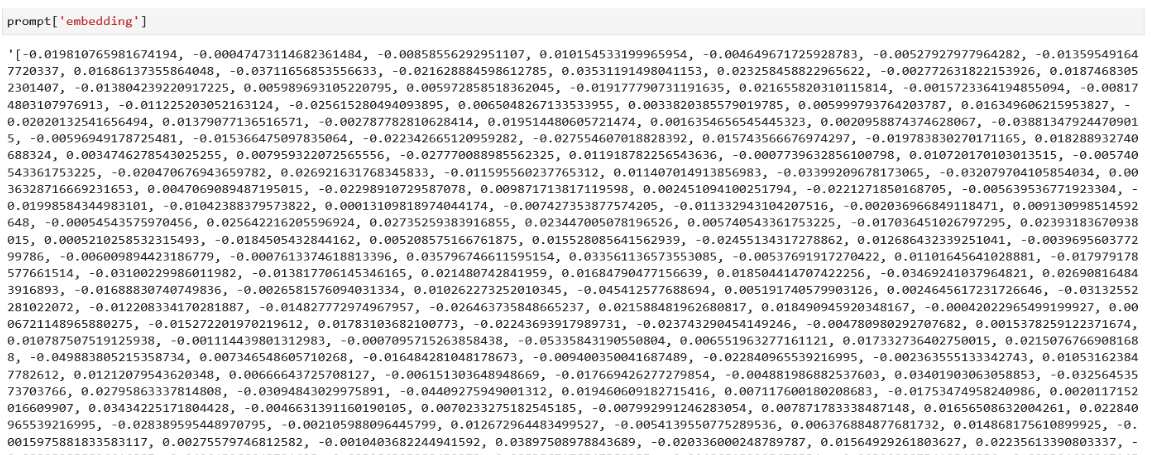
\includegraphics[width=0.7\textwidth]{figures/embedding1.png}
    \caption[Representación vectorial de un prompt luego de pasar por la funcion de embedding]{Representación de un prompt luego de pasar por la funcion de embedding 'text-embedding-ada-002'\\
    {\scriptsize (Fuente: Elavoración propia)}}
    \label{fig:caso1}
\end{figure}


Una vez calculada la similitud coseno entre el vector asociado al prompt y los vectores que presentan los documentos que se encontraban en la 
base de datos, se procede a elaborar un ranking de los documentos más relevantes, según la similaridad obtenida del cálculo de similitud de cosenos. 
Esto se realiza seleccionando los 'n' documentos con los valores de similitud más altos, siendo en el ejemplo proporcionado un total de 3 
presente en la \autoref{fig:caso2}.

\begin{figure}[ht!]
    \centering
    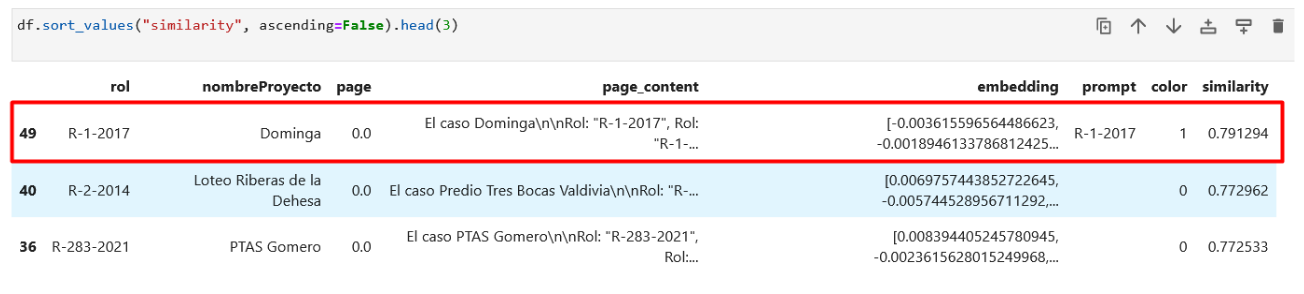
\includegraphics[width=1\textwidth]{figures/embedding2.png}
    \caption[Screenshot de un jupyter notebook representando el proceso interno de selección]{Screenshot de un jupyter notebook representando el proceso interno de selección\\
    {\scriptsize (Fuente: Elavoración propia)}}
    \label{fig:caso2}
\end{figure}

\newpage

Todo este proceso funciona internamente usando Langchain que consulta estos ‘n’ documentos, siendo en este caso 3, a la base de datos 
ChormaDB y son enviados como contexto dentro del prompt a OpenAI mediante el uso de su API, junto a la key de autorización, 
para obtener el resultado del modelo.

Finalmente, se obtiene el resultado por parte del modelo y es procesado por el frontend de la forma que se observa en la \autoref{fig:caso3}, 
lo que da fin al proceso que realiza el Chatbot de principio a fin.


\begin{figure}[ht!]
    \centering
    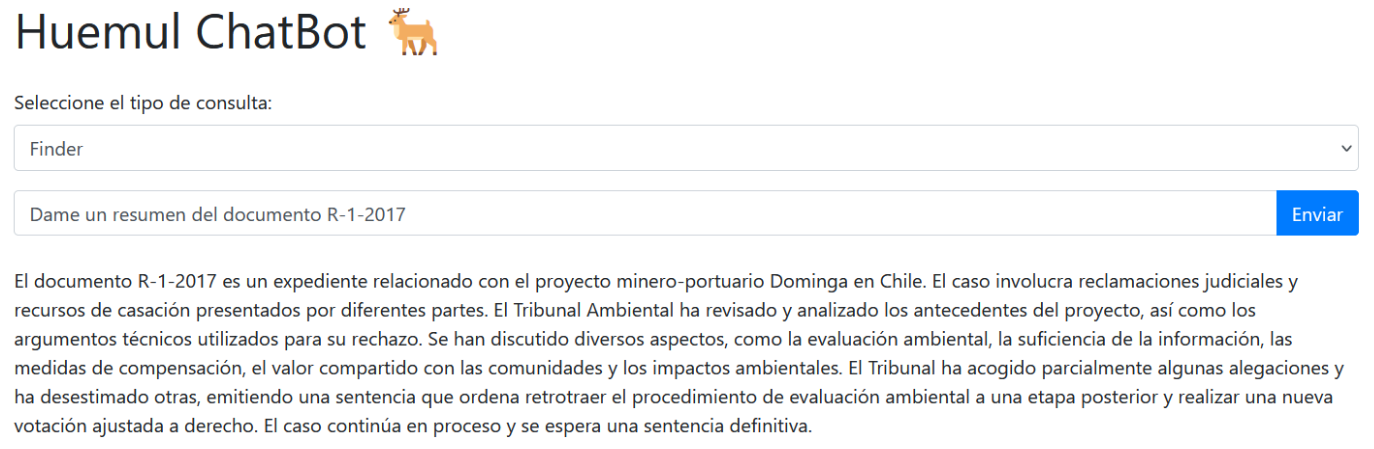
\includegraphics[width=0.95\textwidth]{figures/website2.png}
    \caption[Screenshot del funcionamiento del Chatbot]{Screenshot del funcionamiento del Chatbot\\
    {\scriptsize (Fuente: Elavoración propia)}}
    \label{fig:caso3}
\end{figure}